\section{论文工作是否按预期进行、目前已完成的研究工作及结果}
\subsection{论文工作是否按预期进行}
论文工作按照预期进行: \par
2022.11 - 2022.12: 代码框架搭建完成, 基于相机的SDK开发相机取图进程,实现检测部分的传统算法。\par
2023.01 - 2023.02:实现检测部分的深度学习部分:数据集制作、网络训练、网络部署。\par
2023.02 - 2023.03:实现基于卡尔曼滤波器的追踪和预测部分。\par
\subsection{目前已完成的研究工作及结果}
\subsubsection{检测算法中的传统视觉部分}
传统视觉算法负责的内容是提取出感兴趣的区域,即装甲板区域。总体流程是:二值化图像、提取轮廓、灯条判别、灯条匹配装甲板。
首先为了能去提取装甲板的灯条信息需要先将得到图像进行二值化的处理,因为装甲板左右两侧的灯条的亮度是远高于背景环境的,
所以通过设定一个阈值二值化图像便可以很好的将装甲板的灯条提取出来,但是在测试中发现由于装甲板所处的光照环境不同,
对于二值化阈值的选取有着一定的难度,为了让二值化提取能够更好的适应不同的环境我尝试了以下几种方法:\par
1. 使用全局自适应二值化。\par
2. 使用红蓝通道相减的方法对相减之后的图像进行二值化。\par
3. 使用红/蓝通道进行二值化,同时将原图的灰度图二值化,最后将两张图按位与,得到所需的二值化图片。\par

针对以上三种二值化方案我分别进行了测试,首先第一种全局自适应二值化可以很方便的使用OpenCV内置的api实现,不过通过对大量场景下的测试发现由于部分情况下灯条可能与环境中某一处的灯光所重合,
由于二者亮度相差不大,所以自适应二值化会将二者一同处理,造成最终得到的灯条轮廓不闭合,对之后的轮廓筛选造成影响,所以这个方法的适应性一般。\par

第二种方法是基于OpenCV在图像处理中的特点而实现,OpenCV中如果两张图片相减后得到的像素点的值是小于0的那么会直接让它等于0,
而所需要识别的装甲板的灯条只有红蓝两种形式,若将红蓝两通道相减则可以很好的将灯条信息提取出来,但是由于相机参数的影响,
有时会使得灯条的中部为白色,这样的话对应位置红蓝两通道的值相差便不大,
相减之后得到的值几乎为0,二值化之后得到的灯条图像就不再是一个类似矩形的形状,而是一个圆环状,这种情况下也是可能出现轮廓不闭合的问题,导致之后的轮廓提取出现问题。\par

第三种方案通过众多的测试发现在多种情况下都能比较不错的实现对于灯条的提取,
通过分析可以发现由于使用的是灰度图像所以对于场地颜色还有亮度的适应性更强,结合对于颜色通道的二值化图像可以较好的得到最终所需的二值化图像。\par

经过了二值化之后所有亮度高于灯条或者与灯条亮度一致的区域都会被保留下来,需要通过筛选将一些明显不符合灯条特征的区域筛去。\par

首先找出图像中所有的轮廓,然后通过OpenCV中拟合矩形的两种的方式(minAreaRect、fitEllipse)获取所有轮廓的外接矩形,
获取外接矩形后便拥有了它们的长宽以及角度信息,这样便可以利用轮廓的长宽比以及它们的角度进行一个初步的筛选,将满足条件的装甲板存储起来进行下一步的判断。\par

在得到了所有的可能的灯条后需要将灯条两两匹配,找到属于每个装甲板的那组灯条,装甲板为一个很标准的矩形,尽管视野中装甲板的距离、角度等都会有所不同,
但是两根灯条之间的相关参数都还是处于一定范围之内的,通过判断两根灯条的x、y方向上的距离、长宽比、倾斜角度、角度差
等信息得到满足装甲板条件的一对灯条,得到了这对灯条的信息后其实也就得到了对应装甲板的各类信息,便于后续计算的使用。\par
如下图所示,传统图像处理算法提取中多个可能存在装甲板的ROI。

\subsubsection{检测算法中的深度学习部分}

为了防止出现误识别的情况,提取到“装甲板”对应的ROI区域后需要将它们放入分类器去进行分类,此外对于不同的兵种(装甲板对应不同的数字)击打的优先级是不同的,因此对于装甲板类别的判断是非常重要的。\par
目前对于图像分类的方式有许多种,比如基于卷积神经网络方案和传统机器学习(如SVM)等。我们要做的是对装甲板分类,装甲板的特征比较简单但是类别较多,同时还需要具备对于负样本的判断能力,
基于这几个特点我们选用了带残差层的全连接神经网络。全连接的神经网络虽然形式简单同时也能获得一个较高的准确度,
但是全连接层巨大的参数量会对运行时间造成很大的影响,因此我们考虑使用全局平均池化去解决参数量大的问题,
可使用全局平均池化虽然减少了参数量却丢失了许多信息,测试发现模型收敛后很难达到一个较高的准确度。
对于此问题我们所采用的解决方案是在两层卷积层之后引入一个残差块,将前两层卷积所提取到的特征信息与第三层卷积层的计算结果融合起来,
然后再去使用全局平均池化,经过测试发现最终它所能达到的准确甚至是可以略微超过单纯的全连接神经网络,具体网络结构如下:\par
\begin{figure}[H]
    \centering
    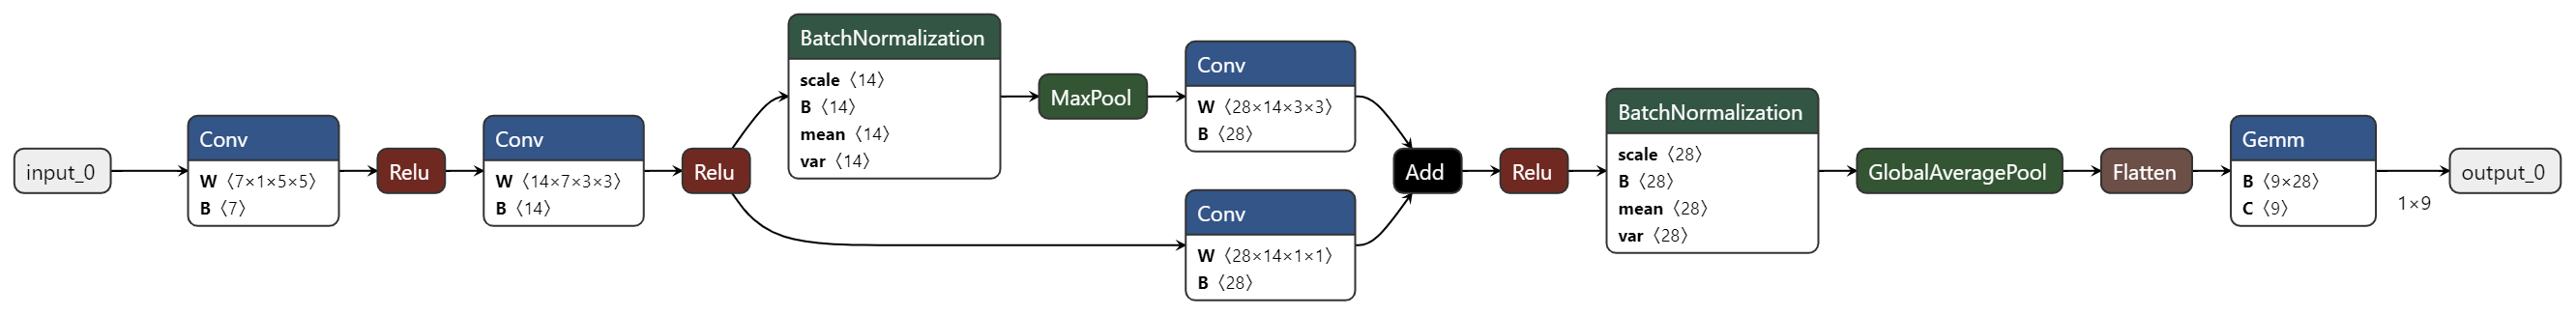
\includegraphics[width=.8\textwidth]{classify_network_structure.png} %1.png是图片文件的相对路径
    \caption{分类器网络结构} %caption是图片的标题
\end{figure}

下图展示训练时的准确率、LOSS值的变化以及ROC曲线绘制。
\begin{figure}[H]
    \centering
    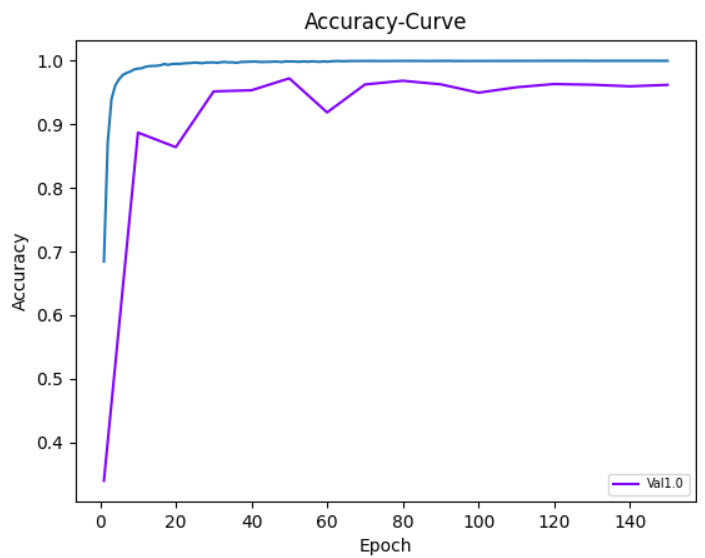
\includegraphics[width=.8\textwidth]{train_accuracy.png} %1.png是图片文件的相对路径
    \caption{训练时准确率变化} %caption是图片的标题
\end{figure}

\begin{figure}[H]
    \centering
    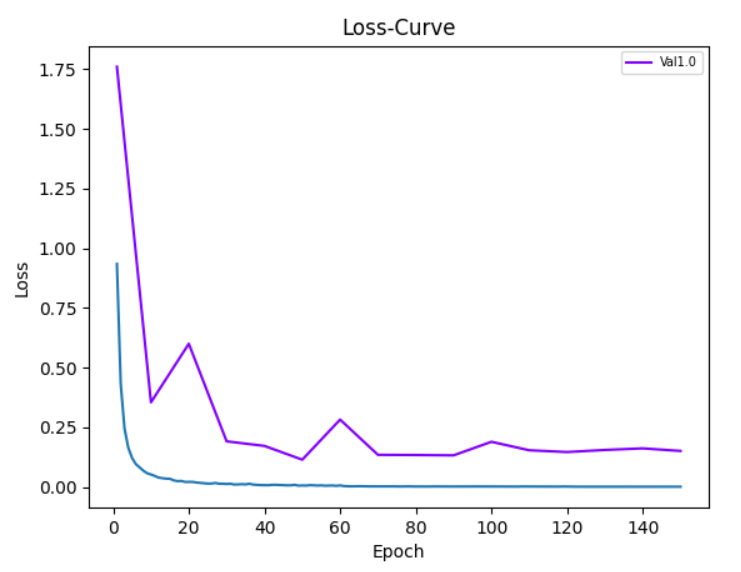
\includegraphics[width=.8\textwidth]{train_loss.png} %1.png是图片文件的相对路径
    \caption{训练时LOSS值变化} %caption是图片的标题
\end{figure}

\begin{figure}[H]
    \centering
    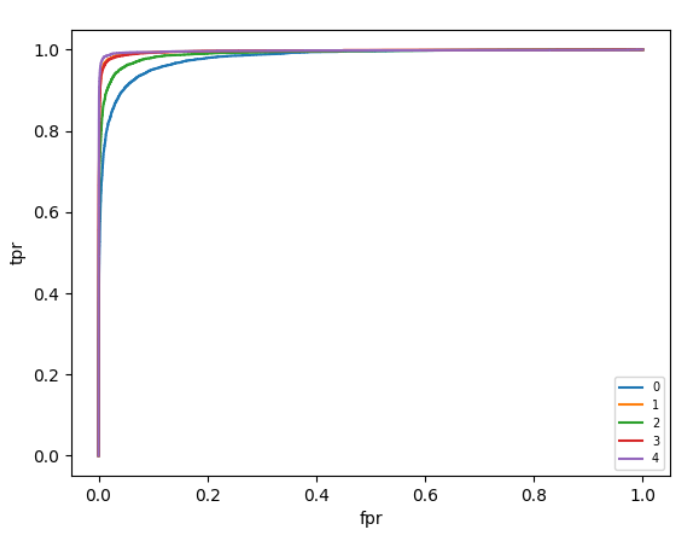
\includegraphics[width=.8\textwidth]{train_ROC.png} %1.png是图片文件的相对路径
    \caption{ROC曲线} %caption是图片的标题
\end{figure}

下图展示训练后的神经网络在面对新数据时的表现。
\begin{figure}[H]
    \centering
    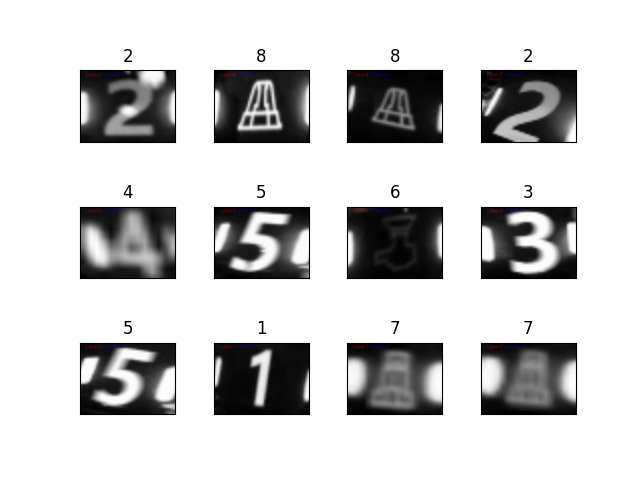
\includegraphics[width=.8\textwidth]{classify_demo.png} %1.png是图片文件的相对路径
    \caption{分类器测试结果} %caption是图片的标题
\end{figure}

下图为,经过分类器判别之后得到的装甲板。
\subsubsection{运动预测算法}






\section{后期拟完成的研究工作及进度安排}
\subsection{后期拟完成的研究工作}
1. 完成单目相机测距算法。\par
2. 完成受空气阻力的弹道迭代计算。\par
3. 充分测试系统的鲁棒性,如识别算法在不同光照环境下的表现效果,预测算法在角度跨圈时处理是否得当,滤波算法是否能够很好的应对不同的噪声。\par
4. 与控制系统联合调试,测试实际效果。\par
\subsection{后期进度安排}
以上(后期拟完成的研究工作)均在2023.04月份完成。
\section{存在的问题与困难}
1. 赛场环境非常复杂,而图像预处理的二值化操作严重依赖于阈值的选择。相同曝光时间下,因环境亮度不同, 二值化阈值也不同,
需要设计硬件自动曝光与软件自动曝光算法,使得在不同光照环境下得到的图像亮度基本保持一致。\par

2. 数字识别在低亮度环境下表现效果不好。因为要追求高帧率的目标检测,假设目标帧率为 150fps,
则最大曝光时间不超过6.7ms,在弱光照环境下成像较暗,卷积分类网络表现效果不好。针对此问题,计划通过两种方式解决:
- 增加在此光照环境下的数据集,让神经网络多学习这一场景。
- 由于数字图案的背景都是黑色的,而数字本身是白色的,通过大津二值化算法实现数字与背景的图像分割,让数字图案更加清晰,数字特征更加明显。\par
\section{论文按时完成的可能性}
论文能够保证按时完成,主要技术问题都得到解决,剩下的只是一些小的细节和优化。\par
\section{参考文献}
\bibliographystyle{hithesis}
\bibliography{reference}

% Local Variables:
% TeX-master: "../mainart"
% TeX-engine: xetex
% End: